% !TEX root = memoire.tex

\section{Terrain d'étude}

\subsection{Présentation du fonds}


La bibliothèque du musée d'Orsay, aussi nommée officiellement « bibliothèque de conservation », est une bibliothèque de recherche spécialisée appartenant à l'établissement public des musées d'Orsay et de l'Orangerie \footcite{reseaubibart}. 

Constituée dès 1975, lors de la préfiguration du musée, elle a pour principale mission d'accompagner et de soutenir le travail scientifique des équipes du musée, mais aussi du corps académique ou de recherche. Elle est ouverte aux étudiants et chercheurs extérieurs sur inscription.


Cette fonction de recherche est une mission centrale de l'institution. La bibliothèque a eu un rôle fondateur lors de sa préfiguration entre 1976 et 1986, que ce soit pour la préparation des grandes expositions inaugurales ou dans sa mission d'archivage du bâtiment en lui-même.

Ses collections comptent plus de 50 000 monographies et 600 titres de périodiques\footcite{museeorsay} . Elles comprennent des ouvrages précieux et rares, comme les catalogues de salons et d'expositions universelles, qui sont des éditions originales illustrées par des artistes. On y trouve aussi un fonds documentaire composé de publications scientifiques anciennes ou récentes, internationales, ainsi que des thèses et mémoires portant sur les artistes, les courants ou les thèmes de l'époque spécialisée du musée, et notamment les travaux lauréats du prix du musée d'Orsay.

Les collections de la bibliothèque du musée d'Orsay sont le résultat du regroupement d'ouvrages provenant de plusieurs institutions, comme la Bibliothèque centrale des musées nationaux (alors physiquement située au Louvre), le musée de l'Orangerie, le musée du Jeu de Paume et le musée national d'art moderne, alors installé au Palais de Tokyo avant l'ouverture du Centre Pompidou. En un seul lieu, la bibliothèque du musée d'Orsay rassemble ainsi une documentation spécifique de la période 1848-1914.


Elle ouvre habituellement ses portes du lundi au vendredi de 14 h à 17 h 30 sans rendez-vous, mais elle reste fermée jusqu'en 2027 afin de préparer l'ouverture du nouveau centre de ressources et de recherche\footcite{ccfr}.



\subsection{Volumétrie et état des données}

Le corpus de ce projet de déménagement et de reclassification est d'environ 50 000 ouvrages spécialisés sur la période 1848-1914.
La bibliothèque utilise un système de cotation développé en interne, attribué à l'ensemble des fonds. Ce système encode le domaine (comme « P » pour peinture ou « S » pour sculpture).

Les données exploitées par le pipeline proviennent du système intégré de gestion de bibliothèque (SIGB) Syracuse, qui héberge l’ensemble des notices du catalogue. L’extraction se fait par export au format CSV via le module de recherche Archimed. Les champs disponibles dans cet export correspondent aux données mobilisées : titre, cote Orsay (ancienne cote interne) existante, ISBN lorsqu’il est renseigné, et sujets RAMEAU lorsqu’ils ont été indexés.

Parmi ces documents, environ 16 à 17 \% du fonds possède un ISBN, une proportion qui permet d'envisager une récupération directe des cotes LC déjà attribuées par d'autres bibliothèques.

Les notices RAMEAU constituent un autre élément important des données. Ce sont des notices d'autorité matière qui regroupent certains mots-clés : noms communs (associés à certains noms propres), noms géographiques, subdivisions chronologiques, titres de publications en série, personnages fictifs ou vedettes de noms de personnes. Leur fonction est de classer hiérarchiquement certaines catégories de notices et de former un ensemble de descripteurs pour l'indexation. \footcite{rameaubnf}

Le champ RAMEAU est présent dans la grande majorité des notices, mais avec une qualité assez hétérogène : certaines sont riches de vedettes précises, tandis que d'autres sont lacunaires. Les limites de cette hétérogénéité fait l'objet de tests dans la troisième partie de ce mémoire.



\subsection{Le système de cotation actuel}

Le système de cotation local de la bibliothèque du musée d'Orsay est désigné sous le nom de cote Orsay (inspiré de la cotation Clément). Non standardisé, ce système structure la cote en trois éléments : le format physique du volume, une ou deux lettres encodant le domaine thématique, et un numéro d'ordre d'entrée dans la collection.

Une cote telle que « 4P72 » se décompose en un format « 4 », un domaine « P » pour Peinture et un numéro d'entrée « 72 ».

\begin{table}[htbp]
\centering
\small
\setlength{\tabcolsep}{4pt}
\renewcommand{\arraystretch}{0.9}
\begin{tabular}{@{}p{0.1\textwidth}p{0.35\textwidth}p{0.1\textwidth}p{0.35\textwidth}@{}}
\toprule
\textbf{Cote} & \textbf{Catégorie} & \textbf{Cote} & \textbf{Catégorie} \\
\midrule
A      & Architecture                                   & Q       & Catalogues commerciaux, Manuels techniques \\
B      & Monographies d'artistes                        & R       & Généralités \\
C      & Cinéma                                         & S       & Sculpture \\
D      & Dessin, Arts graphiques, Pastel, Gravure, Affiches & T   & Marché de l'art, Collections, Collectionneurs, Marchands, Catalogues de vente \\
E      & Expositions                                    & UP      & Recherche de Provenance \\
ES     & Salons                                         & U -- UV & Musées : muséographie, muséologie, études des publics, ... \\
EU     & Expositions universelles                       & UBib    & Bibliothèque ouvrages professionnels \\
F      & Photographie                                   & VO      & Musée d'Orsay : histoire et collections \\
G      & Gastronomie, Arts de la table, Histoire de l'alimentation & VLOU & Musée du Louvre \\
H      & Histoire                                       & VLUX    & Musée du Luxembourg \\
I      & Imprimerie, Edition                            & VP      & Musées parisiens \\
J      & Journalisme, Presse                            & VF      & Musées français, autres que Paris \\
K      & Critique artistique et littéraire              & W       & Musées étrangers \\
L      & Objets d'art                                   & X       & Périodiques, Catalogues de ventes (abonnements jusqu'en 2014) \\
M      & Musique, Théâtre, Spectacles                   & Z       & Usuels (Dictionnaires, Répertoires, etc.) \\
P      & Peinture                                       &         & \\
\bottomrule
\end{tabular}
\caption{Table de correspondance Cote Orsay locale}
\label{tab:cote-orsay}
\end{table}

\subsection{Le projet de reclassification vers LC}

Le projet de reclassement s'inscrit dans la création du futur centre de ressources et de recherche Daniel Marchesseau, dont l'installation est prévue pour la fin 2027 dans l'hôtel de Mailly-Nesle. Ce déménagement inclut notamment un changement dans sa politique d'accès. L'inscription restera obligatoire, mais la majorité de la collection sera proposée en libre accès sur les rayonnages : aujourd'hui, seuls les conservateurs et documentalistes peuvent aller chercher directement un ouvrage en rayon, les lecteurs devant passer par le personnel ; demain, les lecteurs inscrits pourront s'y servir eux-mêmes directement\footcite{cadrageprojet}.

Cette décision de libre accès pose la question du passage d'un classement local spécifique à la bibliothèque du musée d'Orsay à un classement plus standard et plus intuitif. Une cote locale peut devenir un frein à l'autonomie du public, mais aussi à l'autonomie des personnes qui sont moins familières avec les collections de la bibliothèque.

Avec un changement de classification la difficulté est de savoir comment choisir une nouvelle classification adaptée à ses objectifs. 

Sur le plan pratique, l'Institut national d'histoire de l'art (INHA) a implémenté dans une partie de sa collection la classification \textit{Library of Congress}. Cela facilite l'interopérabilité au sein du réseau Bibart, mais aussi l'accès aux ouvrages pour le public. La \textit{Library of Congress}  offre une sélection plus fine au niveau du domaine artistique et de l'histoire de l'art. 


Un autre élément de nature plus éthique que structurelle a pesé dans la décision de la bibliothèque du musée d'Orsay (voir Partie 1, \S\ref{sec:lcc-histoire}).
La figure de Melvil Dewey a en outre été récemment remise en cause en raison de ses prises de position racistes et antisémites, ainsi que d'accusations et de condamnations pour des faits de violence sexiste et sexuelle. L'\textit{American Library Association} a notamment pris position en retirant son nom d'une des distinctions qu'elle attribue\footcite{ala2019}.D'un point de vue structurel, le système Dewey présente lui aussi un biais documenté :une part écrasante des divisions de la classe religion est consacrée au christianisme. Il convient cependant de noter que la \textit{Library of Congress} n'est pas exempte de critiques similaires : plusieurs études relèvent une répartition inégale de l'espace de classification entre traditions religieuses, notamment entre christianisme et islam, ainsi que d'autres catégories ethnocentriques dans ses propres schémas\footcite{bakerislam2020,knowlton2005}. Plus largement, la LCC reste par essence un système très américano-centré, conçu à l'origine pour organiser les collections de la plus grande bibliothèque des États-Unis, ce dont hérite en partie ce type de déséquilibre. Le choix de la LCC ne prétend donc pas à une neutralité absolue face à ces enjeux.


Cette dimension ouvre une question plus large qui dépasse le cadre de ce projet : la charge et la responsabilité éthique de tout système de classement, et la façon dont il peut perpétuer ou invisibiliser certaines réalités. Ce mémoire ne prétend pas trancher cette question, mais les choix méthodologiques qui structurent ce travail peuvent s'y lire comme une réponse pratique et modeste : le plan de cotation curaté par la bibliothèque plutôt qu'un import brut du barème LCC complet (voir \S\ref{sec:niveau2}), et la vérification humaine systématique proposée dans le \textit{workflow} final (voir Partie 3, \S\ref{sec:workflow}), refusent qu'un système de classement s'impose tel quel, sans que l'institution documentaire garde la main sur la façon dont son propre fonds est représenté.

\section{Architecture du pipeline en cascade}


C'est dans l'esprit de donner à la bibliothèque la maîtrise de son propre périmètre de classification plutôt que de lui imposer un système clé en main  que s'est construite l'architecture technique présentée dans cette section.

Le principal défi de cette transition, et notamment de la commande institutionnelle, est d'identifier un équivalent ou un indice de la cotation LC. La méthode explorée est celle de restreindre les cotes disponibles à partir du plan de cotation sélectionné par la bibliothèque, de recourir à une intelligence artificielle pour les cas non résolus par les étapes précédentes, et de réaliser un bilan des opérations de recotation.


Pour cela, une architecture en cascade a été mise en place. Le principal but et la logique de cette architecture en cascade est d'éviter le recours à un grand modèle de langage (LLM) si une méthode plus efficace est possible, c'est-à-dire si une méthode déterministe est possible. Le LLM n'intervient principalement que dans les cas où l'automatisation avec des règles est limitée. L'architecture se constitue en plusieurs niveaux et identifie les différentes catégories d'œuvres pour les traiter différemment, si possible.
Sur le plan technique, l'ensemble du pipeline est développé en langage Python, et s'exécute dans un environnement Google Colab, choisi pour sa gratuité et l'absence de configuration matérielle requise (voir Partie 3, \S\ref{sec:reproductibilite-gpu}). 

\begin{figure}[H]
  \centering
  \makebox[\textwidth][c]{%
    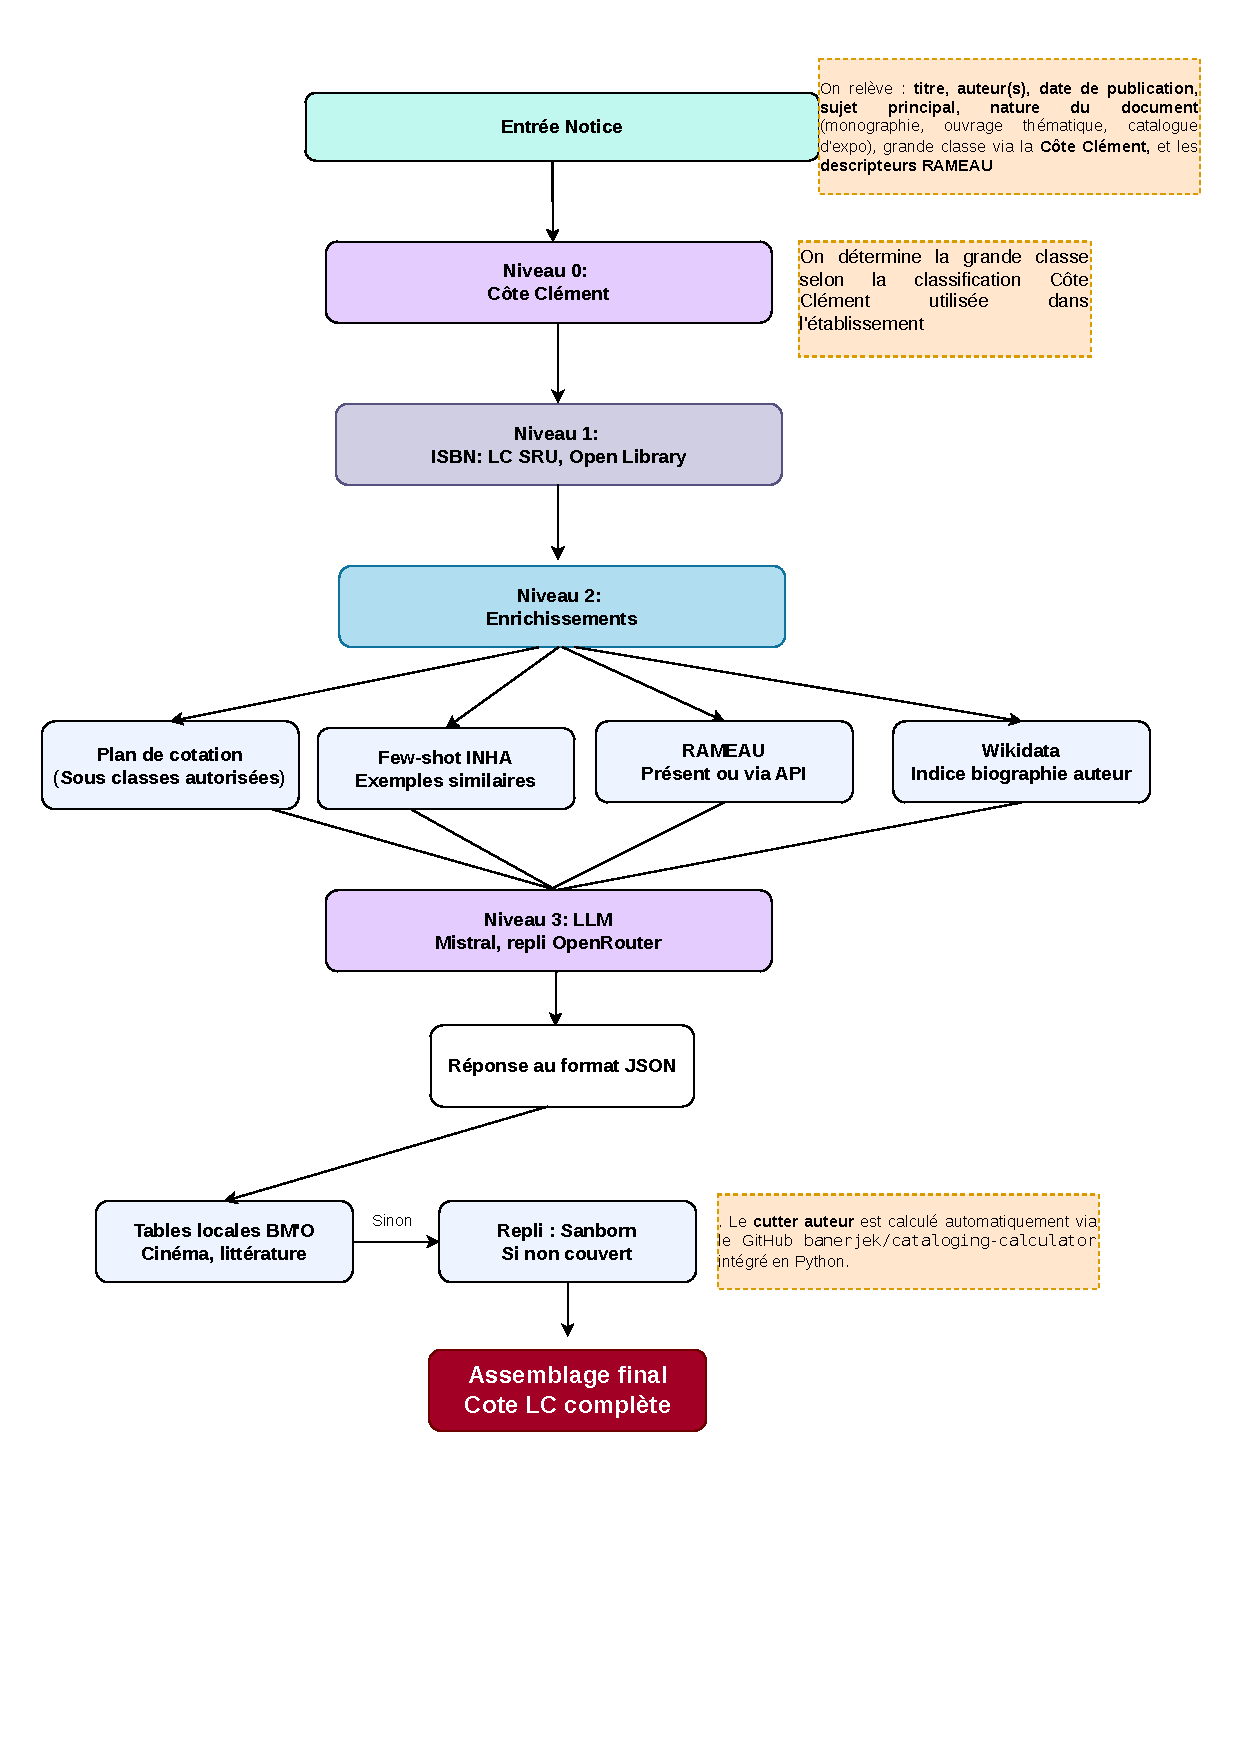
\includegraphics[width=0.85\textwidth]{schema_pipeline_cascade.pdf}%
  }
  \caption{Architecture du pipeline en cascade}
  \label{fig:pipeline}
\end{figure}


\subsection{Niveau 0 : grande classe via Cote Orsay interne}
\label{sec:niveau0}

Le \textit{pipeline}  de la cotation automatisée va se composer de plusieurs étapes successives. La première va consister en un simple dictionnaire pour déterminer la grande classe LC (par exemple, N pour les beaux-arts) à partir de la cote Orsay locale existante. Ce choix a été fait pour faciliter le travail du LLM et parce que c'était une étape qui pouvait être automatisée. La liste des grandes catégories est facilement traduisible en LCC.

Cette étape va restreindre le périmètre des classes autorisées dans le plan de cotation de la bibliothèque du musée d'Orsay et fournir au LLM un contexte cadré pour  choisir une sous-classe plus pertinente. La méthode est déterministe : la lettre Orsay (issue de la cotation locale) est traduite en grande classe \textit{Library of Congress} par une table de correspondance. Le coût en appel LLM est nul et ce socle déterministe est ce qui rend le reste du pipeline possible, puisqu'il libère les niveaux suivants de la charge d'identifier la grande classe pour se concentrer entièrement sur la sous-classe.

La difficulté ne se situe pas au niveau de la grande classe, où une étape conversion simple entre grandes classes est possible, mais au niveau de la sous-classe, là où la classification reste plus difficile à déterminer. C'est donc le LLM qui doit arbitrer entre la plausibilité formelle ou la pertinence sémantique. Ce choix a été fait pour exploiter l'ancienne cote Orsay locale, sécuriser la grande classe et concentrer l'effort de recherche là où se manifestent les limites de l'automatisation.





\begin{lstlisting}[caption={Extrait de la table de correspondance Cote Orsay (niveau 0)}, label={lst:correspondances}]
CORRESPONDANCES_ORSAY = {
    "P": "ND",   # Peinture
    "S": "NB",   # Sculpture
    "E": "N",    # Expositions
    "F": "TR",   # Photographie
    "UV": "AM",  # Musees
    # ...
}
\end{lstlisting}

\subsection{Niveau 1 : recherche par ISBN}
\label{sec:niveau1-isbn}

Une fois la première étape passée, c'est-à-dire la détermination de la grande classe, une deuxième étape vise à enrichir les données le plus possible avant de les fournir au LLM. Cette étape consiste à enrichir la notice d'information pour le LLM.

Elle repose sur l'interrogation de l'ISBN de l'ouvrage auprès de deux sources complémentaires : le service SRU de la \textit{Library of Congress}, puis, en cas d'échec, l'API Open Library.

Cette double interrogation nous donne une couverture combinée d'environ 48\%  des notices possédant un ISBN. 

Le choix de chercher l'ISBN s'appuie sur le script  de Melissa Belvadi\footcite{belvadi2023}, qui interroge les catalogues de Harvard, Stanford et Yale pour retrouver une cote LC déjà attribuée à un ISBN donné, avec un cache local SQLite évitant de solliciter inutilement les serveurs distants pour les ISBN déjà recherchés.



\subsection{Niveau 2 : enrichissement des métadonnées}
\label{sec:niveau2}


Dans la même logique que la recherche par ISBN, cette étape vise à enrichir les métadonnées de la notice avant de solliciter le LLM. Soit les sujets RAMEAU sont déjà présents dans les données initiales fournies à l'outil, soit ils sont recherchés via des appels API pour enrichir ces métadonnées. Une priorité est accordée aux sujets RAMEAU plutôt qu'au titre. Le titre peut en effet être trompeur : par exemple, un ouvrage intitulé « Musée Gaumont » peut traiter de cinéma et non de muséologie, tandis que les vedettes RAMEAU définissent les véritables sujets intellectuels de l'ouvrage.

Le plan de cotation est ensuite injecté dans le prompt. C'est un plan qui a été validé par l'équipe de la bibliothèque. Le LLM ne reçoit que les sous-classes de la grande classe déjà identifiées et extraites de ce plan. Deux sources l'alimentent : les plans détaillés fournis par l'équipe de la bibliothèque pour les domaines spécifiques et le plan générique LCC en JSON pour les autres domaines.


Cette étape d'enrichissement, dont nous testerons la validité, a pour objectif de donner le plus de chances possible au LLM de choisir la sous-classe la plus pertinente, grâce aux sujets RAMEAU et à l'enrichissement \textit{few-shots}.



\subsection{Niveau 3 : proposition par le LLM}
\label{sec:niveau3-llm}


Le \textit{pipeline}  utilise principalement le modèle Mistral NeMo comme fournisseur principal. Ce modèle a été retenu pour son accès facile et gratuit et sa disponibilité via une API REST\footnote{Une API REST (\textit{Representational State Transfer}) est un style d'architecture standard pour l'échange de données entre logiciels par le protocole HTTPS : chaque requête est autonome et transmise sous une forme normalisée, ce qui la rend indépendante du langage de programmation utilisé de part et d'autre.}.

Le recours à un LLM à ce niveau précis de la cascade, plutôt qu'à une méthode déterministe comme aux niveaux précédents, se justifie par la nature même de la tâche restante : le choix d'une sous-classe pertinente exige un jugement sémantique sur le contenu du document, pour lequel aucune règle simple ne suffit (voir §\ref{sec:justification-architecture}).

Le mécanisme de bascule fonctionne notice par notice, à la suite d'échecs de service rencontrés au cours du développement. Le pipeline tente d'abord Mistral et en cas d'échec distingue deux types d'erreurs. Des erreurs transitoires (comme un quota dépassé), qui déclenche une nouvelle tentative après un délai d'attente, et des erreurs définitives (authentification refusée, accès non autorisé au modèle), qui déclenche une bascule vers un autre fournisseur, OpenRouter. Si les deux fournisseurs échouent l'un après l'autre pour une même notice, le processus s'arrête en sauvegardant la notice.

Les deux services sont interrogés par appel HTTPS direct plutôt que par un kit de développement logiciel tiers (\textit{SDK}), pour trois raisons. Eviter d'installer et de maintenir une dépendance supplémentaire par fournisseur, alors que l'environnement Colab repart de zéro à chaque session. Ensuite, permettre de traiter Mistral et OpenRouter de façon strictement identique dans le code, avec un seul mécanisme de gestion des erreurs (voir plus haut), plutôt que d'adapter la logique de bascule à deux SDK différents, avec chacun ses propres conventions. Enfin, l'appel direct donne un accès complet et sans intermédiaire au code de statut et au contenu exact de chaque réponse, nécessaire comprendre les messages d'erreurs.


La température du modèle, le paramètre qui contrôle le degré de variation aléatoire dans la réponse générée, a été fixée à 0,1, une valeur assez basse. Cela signifie que pour une même notice interrogée plusieurs fois, le modèle produit des réponses identiques ou très proches.
C'est une condition nécessaire pour produire des résultats reproductibles d'une exécution à l'autre, et elle facilite le travail des bibliothécaires ou des personnes qui utilisent l'outil pour obtenir des résultats identiques pour chaque notice.
Le prompt envoyé au modèle assemble plusieurs éléments, chacun avec un but spécifique. D'abord, la grande classe est déjà connue : le modèle n'a pas à la déterminer, il doit juste choisir la sous-classe. Le plan des sous-classes lui est fourni au format CSV (reproduit en annexe) : c'est un plan spécifique déterminé par la bibliothèque du musée d'Orsay, qui délimite toutes les sous-classes possibles et restreint l'espace des réponses à un sous-ensemble pertinent, plutôt qu'à l'ensemble du plan \textit{Library of Congress}.

Ensuite, on appelle une API de l'INHA qui recherche les notices les plus proches par similarité de celle que l'on cherche à coter. On appelle cela du \textit{few-shot}, ce qui montre au modèle un motif concret plutôt qu'une règle abstraite. On lui fournit également une consigne explicite de prioriser les sujets RAMEAU plutôt que le titre. 

Le \textit{prompt}  demande enfin une réponse limitée à la seule cote au format JSON, afin qu'elle puisse être exploitée automatiquement dans la suite du \textit{pipeline} . Le LLM ne produit que la sous-classe : une décision prise pour se concentrer sur ce point plus sensible et plus sujet à l'erreur, plutôt que sur la grande classe.


\subsection{Justification des choix architecturaux}
\label{sec:justification-architecture}

\subsubsection*{L'architecture en cascade comme réponse aux limites des LLM}

L'idée de l'architecture du pipeline résulte d'une réponse aux limites des grands modèles de langage identifiées précédemment. Le but était de mettre en situation l'instruction générative  (\textit{prompting}) du LLM de bout en bout, mais le recours à un LLM sur l'architecture entière présenterait trois problèmes majeurs.

Le premier problème est d'ordre économique et temporel. Chaque appel à un LLM est coûteux, long et peut induire des erreurs si tout repose sur lui. À l'inverse, les niveaux déterministes précédant l'appel au LLM facilitent le travail et donnent plus de chances d'obtenir un résultat correct, plus rapide et moins coûteux. Sur un corpus de 50 000 notices, la différence est considérable.

Une logique de cascade va concentrer le traitement coûteux uniquement sur la partie la plus difficile, c'est-à-dire les étapes qu'on ne peut pas résoudre automatiquement. Cela rejoint un principe de conception bien ancré dans l'apprentissage automatique, notamment popularisé par les détecteurs en cascade \footcite{violajones2001}: plusieurs étapes de classifieurs, du moins coûteux au plus coûteux, filtrent progressivement les cas à traiter pour ne réserver le traitement complexe qu'à la minorité de cas non résolus précédemment. La différence est que les niveaux de ce pipeline de cotation répondent à des questions différentes (grande classe, cotes par ISBN, sous-classe) et fonctionnent plutôt comme une chaîne de méthodes de secours que comme un raffinement progressif. Mais le principe reste d'économiser le calcul coûteux en le réservant à l'étape la plus difficile.

Le second problème est la fiabilité. On peut utiliser la correspondance avec l'ancienne cotation Orsay pour prédire la grande classe, atteindre 100\% de justesse et ainsi augmenter la précision pour l'étape où le LLM doit trouver la sous-classe. Sans cette étape, un LLM, même contraint par un prompt, a plus de chances de générer des erreurs.

Le troisième problème est la traçabilité. L'architecture de ce \textit{pipeline}  est conçue pour attribuer à chaque côte une source explicite et un niveau de confiance numérique. Un LLM unique de bout en bout offre peu de fiabilité, surtout par \textit{prompting}, concernant l'origine de la réponse. La cascade permet de contraindre le LLM et ses erreurs à une seule étape, pour que l'utilisateur final sache à tout moment d'où vient la cote proposée.


\subsubsection*{Le fine-tuning écarté faute de ressources}
La possibilité d'utiliser le \textit{ fine-tuning}  du modèle au lieu du \textit{pipeline}  a été envisagée mais écartée. Les raisons de ce choix sont matérielles et méthodologiques : le corpus d'entraînement disponible est trop petit et insuffisant pour un \textit{ fine-tuning}  satisfaisant, et l'infrastructure ne dispose pas d'un GPU adapté à cette tâche.

Dans le cas de ce projet, la solution a donc été de s'orienter vers du  \textit{few-shot prompting}, qui constitue un compromis entre performance et contraintes. 


\subsubsection*{La dépendance aux API externes comme fragilité structurelle}

L'architecture du \textit{pipeline}  repose sur un nombre important de services externes : le SRU de la Library of Congress et Open Library pour l'enrichissement par ISBN, les API de recherche RAMEAU, l'API de similarité de l'INHA pour le \textit{few-shot}, et enfin les fournisseurs de LLM Mistral et OpenRouter. Cette multiplication des dépendances constitue une fragilité structurelle du \textit{pipeline}: chacun de ces services échappe au contrôle de la bibliothèque du musée d'Orsay, que ce soit en matière de disponibilité, de quota, de changement de format de réponse ou de suppression pure et simple du service, comme cela a déjà été observé lors des tests de plusieurs sources d'enrichissement par ISBN écartées en cours de projet.

Cette fragilité est d'autant plus sensible que le corpus à traiter est volumineux : sur 50 000 notices, une indisponibilité même brève d'un service peut interrompre un traitement de plusieurs heures. Pour limiter ce risque, un mécanisme de disjoncteur (\emph{circuit breaker}) a été intégré à la boucle de traitement : après cinq échecs consécutifs d'un même service, le pipeline enregistre un point de sauvegarde et interrompt l'exécution plutôt que de poursuivre sur des données dégradées ou de saturer inutilement le service distant. Ce choix ne supprime pas la dépendance, mais il permet de reprendre le traitement là où il s'est arrêté plutôt que de perdre l'intégralité d'une exécution.

Cette architecture pose donc une limite méthodologique à anticiper pour tout déploiement en production : la robustesse du \textit{pipeline}  dans la durée dépendra autant de la stabilité des API tierces que de la qualité du code lui-même.

\subsubsection*{La priorisation RAMEAU, levier puissant mais fragile}

Parmi les enrichissements testés, la priorisation des sujets RAMEAU sur le titre de l'ouvrage semble être le levier le plus déterminant pour orienter le LLM vers la sous-classe pertinente. La nature même du champ RAMEAU,  informe sur le sujet intellectuel  de l'ouvrage, quand le titre peut être trompeur ou allusif.

Ce levier reste toutefois fragile pour deux raisons. D'une part, la qualité du champ RAMEAU est hétérogène d'une notice à l'autre : certaines notices disposent de sujets RAMEAU précises et nombreuses, d'autres sont lacunaires ou absentes, ce qui limite mécaniquement le bénéfice de la priorisation aux seules notices correctement indexées. D'autre part, la performance du \textit{pipeline}  sur ce point dépend directement de la qualité du catalogage antérieur réalisé par la bibliothèque, un facteur externe au \textit{pipeline}  lui-même et non maîtrisable par l'automatisation. Un enrichissement RAMEAU de meilleure qualité en amont, ou une politique de catalogage plus systématique, aurait donc un effet direct sur la performance du \textit{pipeline} , indépendamment de toute amélioration technique de la cascade elle-même.

Cette fragilité illustre une limite plus générale de l'automatisation par LLM dans ce contexte : le \textit{pipeline}  ne peut pas compenser entièrement un déficit de métadonnées structurées en amont, il ne peut qu'exploiter au mieux ce qui est disponible.

\section{Constitution du corpus de référence et limites de la validation}

\subsection{L'absence de vérité terrain à Orsay}
\label{sec:absence-verite-terrain}

Une des réponses apportées à cette contrainte a été de recourir à un corpus provenant de l’INHA, qui a recoté une partie de ses collections au format Library of Congress. Le choix méthodologique retenu pour ce corpus est d’imposer la grande classe telle qu’elle figure dans la cote INHA de référence, plutôt que de la faire dériver du niveau 0 du pipeline (\S\ref{sec:niveau0}) : les notices INHA ne portent pas de Cote Orsay, ce niveau ne peut donc pas y être exercé. Ce choix permet de concentrer l’évaluation sur ce que ce corpus peut effectivement mesurer, à savoir la qualité de la sous-classe proposée par le LLM et l’apport des enrichissements de la cascade, mais il a une conséquence qu’il faut garder à l’esprit dans la lecture des résultats de la Partie 3 : la justesse de la correspondance cote Orsay → grande classe elle-même n’est testée par aucune de ces expériences, et les scores obtenus sur ce corpus ne mesurent donc que le comportement du LLM en aval d’une grande classe supposée correcte, pas la performance de bout en bout du pipeline sur un fonds réel.

L’utilisation du corpus de l’INHA comme banc d’essai présente toutefois des limites qu’il convient de lister. L’INHA a en effet adapté la Library of Congress à ses propres règles et appliqué sa propre politique de cotation, qui diverge des choix retenus à Orsay ainsi que de la cotation classique de la Library of Congress. 

Notamment, elle regroupe sous des sous-classes locales NY et NZ, qui n'existent pas dans la \textit{Library of Congress Classification}, l'ensemble des documents portant sur un même artiste quel qu'en soit le type (écrits et correspondance, catalogues raisonnés, monographies, catalogues d'exposition)\footcite{inhalcc}. 
L'organisation du libre accès en corpus thématiques y a été définie avant la correspondance avec la LCC, et c'est cette dernière qui a été adaptée en conséquence plutôt que l'inverse\footcite{inhalcc}. Les indices attribués par les bibliothèques américaines dont proviennent une partie des notices ne correspondent pas toujours aux classes retenues par l'INHA pour ses propres corpus, ce qui a nécessité des règles de correspondance locales~: des ouvrages sur le christianisme dans son rapport à l'esthétique, normalement classés en religion (BR115.A8), ont ainsi été réorientés vers la section Art (N72.R4)~; une partie des ouvrages sur l'histoire du vêtement, relevant en LCC de la classe Coutumes et folklore (GT), a été reclassée dans les Arts décoratifs (NK), section consacrée à la mode\footcite{inhalcc}. Ces réorientations sont motivées par la cohérence des corpus documentaires de l'INHA plutôt que par la logique disciplinaire de la LCC elle-même. 

 Les cotes \textit{Library of Congress}  de l’INHA ne constituent donc pas une vérité de terrain absolue. D’ailleurs, aucune cote ne constitue une vérité de terrain absolue. Le choix de l’INHA s’est fait en raison de la proximité de ses collections d’art avec celles de la bibliothèque du musée d’Orsay. 
Mais chaque bibliothèque a une politique et une approche différentes pour  établir ses cotes \textit{Library of Congress} , ce qui explique la complexité d’effectuer cette cotation.
Les choix de catalogage sont propres aux institutions, et parfois même au bibliothécaire lui-même, qui juge ce qui est optimal pour ses propres collections.

Le banc d’essai a été étendu depuis les premiers tests. Le corpus de l’INHA est désormais composé d’environ 200 notices couvrant une quinzaine de grandes classes, avec un sous-échantillon portant explicitement sur les 18 classes validées par la bibliothèque du musée d’Orsay. Cet élargissement permet d’assurer une meilleure robustesse statistique et de mettre en évidence un écart de performance potentiel entre les classes couvertes et non couvertes par le plan.


\section{Cadre d'évaluation : le degré de rapprochement}

\subsection{Pourquoi une évaluation binaire est insuffisante}
Dans le cadre de l'évaluation, le constat de départ est empirique. Proposer une cote ND 1345 alors que la cote attendue est ND 1350 n'est pas une erreur aussi grande que de proposer une grande catégorie TR au lieu de ND (TR correspondant à la photographie et ND à la peinture). Dans le premier cas, les deux cotes se situent dans la même catégorie, les paysages, alors que la seconde est une branche complètement différente de l'histoire de l'art.

Une évaluation binaire, c'est-à-dire savoir si la cote est strictement correcte ou non, serait donc une mauvaise manière d'interpréter les résultats. Une évaluation binaire nous donnerait peu d'informations sur le potentiel du LLM, notamment parce que la classification dépend des choix arbitraires du bibliothécaire et de l'institution, mais aussi parce qu'elle traiterait ces deux erreurs à la même échelle.

La classification de texte possède une structure hiérarchique de type arbre : une grande classe, une sous-classe, puis une cote précise. Comme l'a souligné la littérature sur les métriques d'évaluation de classification hiérarchique, une métrique qui ignore la hiérarchie mesure mal la qualité de la prédiction et masque le degré de rapprochement entre la cote attendue et la cote réelle\footcite{kosmopoulos2015,kiritchenko2006}.



\subsection{La distance au plus proche ancêtre commun}
\label{sec:distance-lca}

La méthode choisie dans ce pipeline a été d'établir un score qui va mesurer le degré de rapprochement hiérarchique entre la cote proposée et la cote de référence. Pour cela, on identifie, dans le barème LCC officiel complet (soit environ 497 préfixes de classe en hiérarchie parent-enfant, reconstituée à partir des barèmes PDF originaux de la \textit{Library of Congress}), le nœud le plus spécifique contenant chacune des deux sous-classes, puis on remonte leurs ancêtres jusqu'au plus proche ancêtre commun (\textit{lowest common ancestor},LCA).

La taille de cet intervalle est rapportée à l'étendue totale de la classe, ce qui donne une distance $d$ comprise entre 0 (sous-classes identiques) et 1 (aucun ancêtre commun spécifique au sein d'une même grande classe). 

Cette distance $d$ est ensuite convertie en un score de proximité sur une échelle de 0 à 4, par la formule $\text{score} = 4 \times (1 - d)$.Un score de 4,0 correspond à une sous-classe strictement exacte ($d = 0$), tandis qu'un score proche de 0 traduit une sous-classe hiérarchiquement très éloignée (dans la même grande classe). Lorsque la grande classe proposée diffère de la grande classe attendue, le score est fixé directement à 0,0, sans passer par le calcul de la distance LCA : cette situation est jugée qualitativement différente d'un simple éloignement de sous-classe, puisqu'elle correspond à une branche entièrement distincte de la classification (cf. l'exemple TR/ND en \S\ref{sec:niveau2}).

Le cutter est explicitement exclu de cette mesure : une fois la sous-classe déterminée, le calcul du cutter est une opération mécanique qu'il n'est pas nécessaire d'évaluer sur son inexactitude.




\begin{table}[h]
\centering
\begin{tabular}{ll}
\toprule
\textbf{Score} & \textbf{Signification} \\
\midrule
4,0 & Sous-classe exacte ($d = 0$) \\
$]0\,;\,4[$ & Proximité continue, $\text{score} = 4 \times (1 - d)$ \\
0,0 & Grande classe différente (distance LCA non calculée) \\
\bottomrule
\end{tabular}
\caption{Score de proximité de sous-classe, dérivé de la distance normalisée au plus proche ancêtre commun ($d$)}
\label{tab:score-lca}
\end{table}

\subsection{Méthodologie statistique}
\label{sec:methodologie-stats}

Les comparaisons entre conditions présentées en Partie 3 reposent sur trois outils statistiques, définis ici.

Le test de \textbf{Wilcoxon signé} (\textit{Wilcoxon signed-rank test})\footcite{wilcoxon1945} est un test non paramétrique adapté aux comparaisons appariées~: la même notice, évaluée dans deux conditions différentes. Il compare les rangs des différences observées entre les deux séries plutôt que leurs moyennes directement, ce qui le rend robuste à des distributions non normales (nos résultats étant bimodaux\S\ref{sec:distribution-score}). Un écart est considéré comme significatif au seuil nominal lorsque $p < 0{,}05$.

Les \textbf{intervalles de confiance par bootstrap}\footcite{efron1979} sont utilisés pour les scores par grande classe, où l'effectif est restreint. La méthode ré-échantillonne aléatoirement, avec remise, les scores observés d'une classe (2~000 itérations), pour estimer la variabilité de la moyenne sans supposer une loi de distribution connue. Un intervalle qui ne contient pas zéro indique un écart statistiquement établi~; un intervalle qui contient zéro signale un écart trop faible, ou un effectif trop réduit, pour être distingué du hasard de l'échantillonnage.


\section{Protocole expérimental}

\subsection{Vue d'ensemble des expériences}
\label{sec:vue-ensemble-experiences}

Le protocole isole l'effet de chaque levier de la cascade selon un plan factoriel~: deux plans de cotation (réduit BM'O, officiel complet) croisés avec quatre conditions d'enrichissement, soit huit configurations testées sur le même corpus de 201 notices. Le notebook fourni en annexe présente l'outil de cotation dans sa version de production~; les données brutes issues de l'exécution de ces huit configurations (score par notice et par configuration testée) sont fournies séparément au format CSV, et ont servi de base à l'ensemble des résultats et tests statistiques présentés en Partie 3.

\begin{table}[h]
\centering
\small
\setlength{\tabcolsep}{4pt}
\renewcommand{\arraystretch}{1.15}
\begin{tabular}{@{}p{0.15\textwidth}p{0.40\textwidth}p{0.40\textwidth}@{}}
\toprule
\textbf{Condition} & \textbf{Ce qui change par rapport à la configuration standard} & \textbf{Ce qui est mesuré} \\
\midrule
Standard           & RAMEAU actif, few-shot actif (pool de 26 notices) & Configuration de référence \\
RAMEAU désactivé   & Sujets RAMEAU retirés du \textit{prompt}          & Effet de la priorisation RAMEAU (Partie~3, \S\ref{sec:effet-rameau}) \\
Few-shot désactivé & Aucun exemple fourni au modèle                    & Effet du \gls{fewshot} (Partie~3, \S\ref{sec:effet-fewshot}) \\
Pool élargi        & Pool few-shot porté de 26 à 94 notices            & Effet de la taille du pool (Partie~3, \S\ref{sec:effet-pool-elargi}) \\
\bottomrule
\end{tabular}
\caption{Les quatre conditions testées, chacune sous plan réduit et sous plan officiel complet}
\label{tab:experiences}
\end{table}


Chaque condition isole un seul levier à la fois par rapport à la configuration standard, plutôt que de les cumuler progressivement~: cela permet de mesurer l'effet propre de chaque enrichissement, y compris ses variations selon le plan de cotation utilisé (Partie 3, \S\ref{sec:effet-plan-reduit}), plutôt qu'un effet confondu avec l'ordre dans lequel les leviers auraient été ajoutés.

Le détail du test opposant le plan réduit de la bibliothèque du musée d'Orsay au barème LCC complet est présenté et discuté en Partie 3, \S\ref{sec:effet-plan-reduit}, à partir des données brutes fournies en annexe.